\chapter{Assignment: Clustering}
\label{hw:clustering}

\newthought{Clustering helps to discover groups of data}, for example similar batches, which the user can explore in detail with visualizations and statistics. Use FTO3 data from Dr Reddy’s and group them by Batch using the Pivot Table widget. Use Select Columns to keep only those attributes that are important (for example, process parameters). Put all other attributes in metas.

\begin{figure}[h]
  \centering
  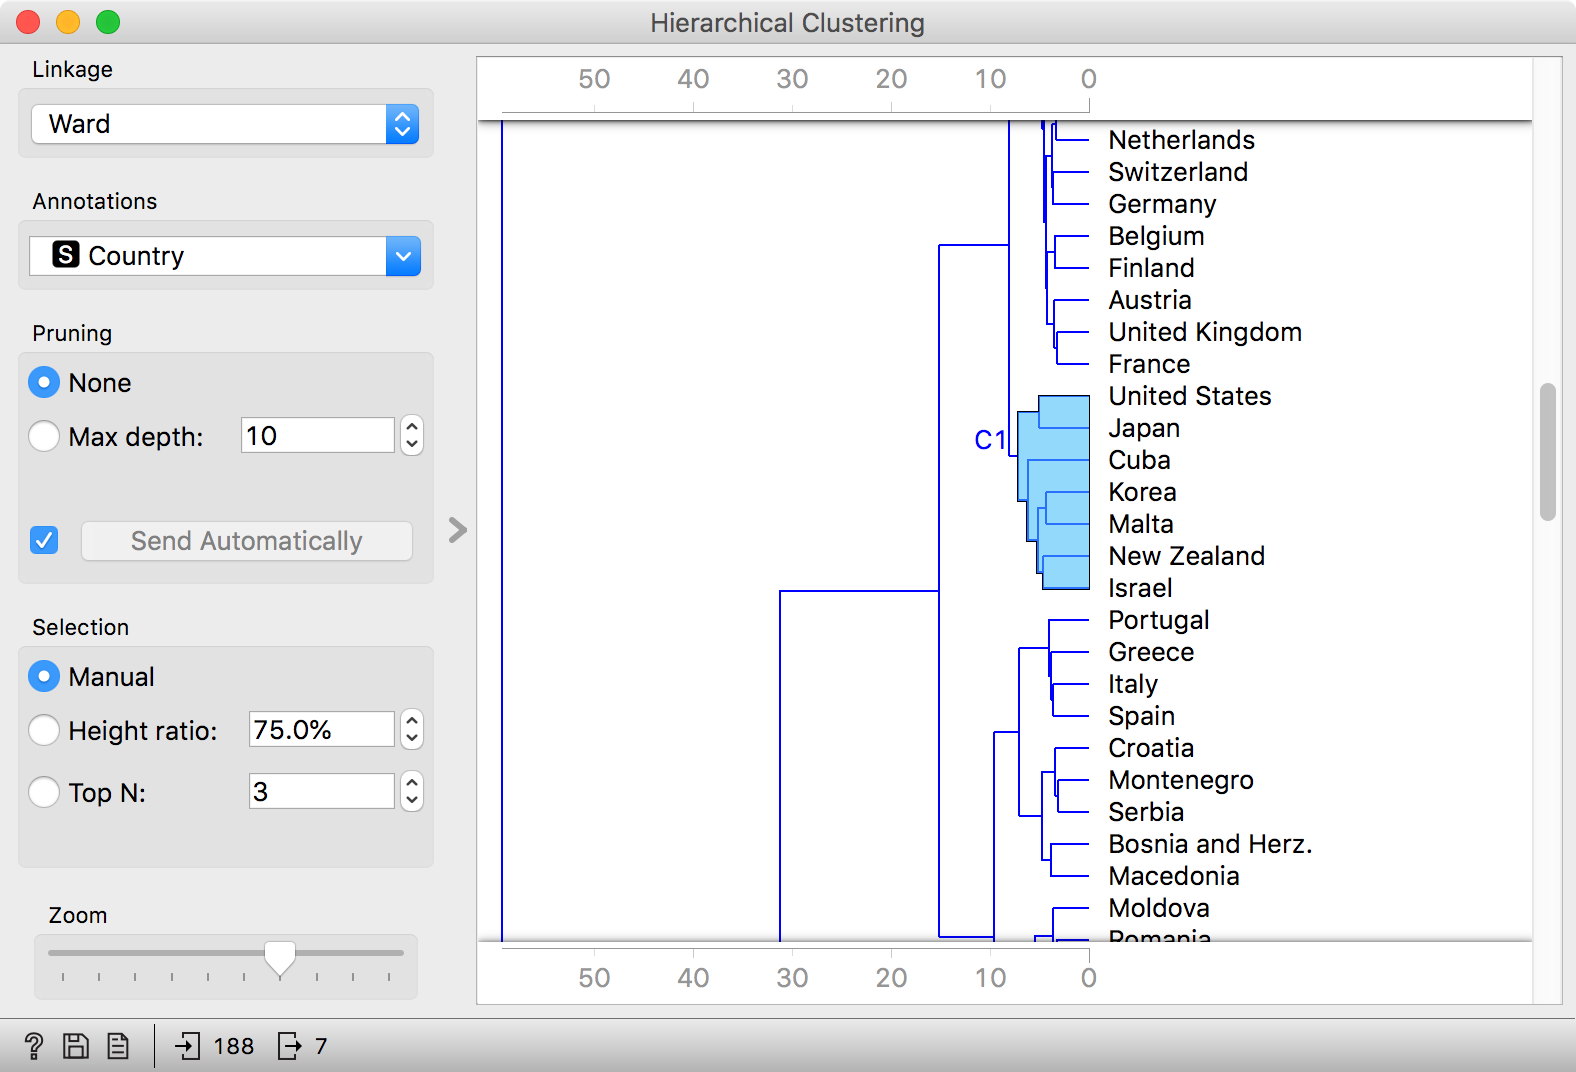
\includegraphics[width=\linewidth]{clustering.png}%
  \caption{Workflow for the assignment.}
  \label{fig:clustering}
\end{figure}

\begin{enumerate}
    \item Try Euclidean and cosine distance with Ward linkage. Which one works better? Why?
    \item How many groups did you discover? What number would make sense?
    \item Explain the final clusters. What defines each of them?
\end{enumerate}
